% Copyright (C) 2014-2016 by Thomas Auzinger <thomas@auzinger.name>

\documentclass[draft,final]{vutinfth} % Remove option 'final' to obtain debug information.

\usepackage{listings}
% Load packages to allow in- and output of non-ASCII characters.
\usepackage{lmodern}        % Use an extension of the original Computer Modern font to minimize the use of bitmapped letters.
\usepackage[T1]{fontenc}    % Determines font encoding of the output. Font packages have to be included before this line.
\usepackage[utf8]{inputenc} % Determines encoding of the input. All input files have to use UTF8 encoding.

% Extended LaTeX functionality is enables by including packages with \usepackage{...}.
\usepackage{float}
\usepackage{fixltx2e}   % Provides fixes for several errors in LaTeX2e.
\usepackage{amsmath}    % Extended typesetting of mathematical expression.
\usepackage{amssymb}    % Provides a multitude of mathematical symbols.
\usepackage{mathtools}  % Further extensions of mathematical typesetting.
\usepackage{microtype}  % Small-scale typographic enhancements.
\usepackage{enumitem}   % User control over the layout of lists (itemize, enumerate, description).
\usepackage{multirow}   % Allows table elements to span several rows.
\usepackage{booktabs}   % Improves the typesettings of tables.
\usepackage{subcaption} % Allows the use of subfigures and enables their referencing.
\usepackage[ruled,linesnumbered,algochapter]{algorithm2e} % Enables the writing of pseudo code.
\usepackage[usenames,dvipsnames,table]{xcolor} % Allows the definition and use of colors. This package has to be included before tikz.
\usepackage{nag}       % Issues warnings when best practices in writing LaTeX documents are violated.
\usepackage{hyperref}  % Enables cross linking in the electronic document version. This package has to be included second to last.
\usepackage[acronym,toc]{glossaries} % Enables the generation of glossaries and lists fo acronyms. This package has to be included last.

% Define convenience functions to use the author name and the thesis title in the PDF document properties.
\newcommand{\authorname}{Kevin Haller} % The author name without titles.
\newcommand{\thesistitle}{Title} % The title of the thesis. The English version should be used, if it exists.

% Set PDF document properties
\hypersetup{
    pdfpagelayout   = TwoPageRight,           % How the document is shown in PDF viewers (optional).
    linkbordercolor = {Melon},                % The color of the borders of boxes around crosslinks (optional).
    pdfauthor       = {\authorname},          % The author's name in the document properties (optional).
    pdftitle        = {\thesistitle},         % The document's title in the document properties (optional).
    pdfsubject      = {Subject},              % The document's subject in the document properties (optional).
    pdfkeywords     = {a, list, of, keywords} % The document's keywords in the document properties (optional).
}

\setsecnumdepth{subsection} % Enumerate subsections.

\nonzeroparskip             % Create space between paragraphs (optional).
\setlength{\parindent}{0pt} % Remove paragraph identation (optional).


\makeindex      % Use an optional index.
\makeglossaries % Use an optional glossary.
%\glstocfalse   % Remove the glossaries from the table of contents.

% Set persons with 4 arguments:
%  {title before name}{name}{title after name}{gender}
%  where both titles are optional (i.e. can be given as empty brackets {}).
\setauthor{}{\authorname}{}{male}
\setadvisor{Ao.Univ.Prof. Dipl.-Ing. Dr.techn. Mag.rer.soc.oec}{Stefan Biffl}{Univ.Doz.}{male}

% For bachelor and master theses:
\setfirstassistant{}{Reka Marta Sabou}{Project Ass.}{female}

% For dissertations:
%\setfirstreviewer{Pretitle}{Forename Surname}{Posttitle}{male}
%\setsecondreviewer{Pretitle}{Forename Surname}{Posttitle}{male}

% For dissertations at the PhD School:
%\setsecondadvisor{Pretitle}{Forename Surname}{Posttitle}{male}

% Required data.
\setaddress{Address}
\setregnumber{1325694}
\setdate{01}{08}{2016} % Set date with 3 arguments: {day}{month}{year}.
\settitle{\thesistitle}{Titel der Arbeit} % Sets English and German version of the title (both can be English or German).
\setsubtitle{Optional Subtitle of the Thesis}{Optionaler Untertitel der Arbeit} % Sets English and German version of the subtitle (both can be English or German).

% Select the thesis type: bachelor / master / doctor / phd-school.
% Bachelor:
\setthesis{bachelor}
%
% Master:
%\setthesis{master}
%\setmasterdegree{dipl.} % dipl. / rer.nat. / rer.soc.oec. / master
%
% Doctor:
%\setthesis{doctor}
%\setdoctordegree{rer.soc.oec.}% rer.nat. / techn. / rer.soc.oec.
%
% Doctor at the PhD School
%\setthesis{phd-school} % Deactivate non-English title pages (see below)

% For bachelor and master:
\setcurriculum{Software and Information Engineering}{Software und Information Engineering} % Sets the English and German name of the curriculum.

% For dissertations at the PhD School:
\setfirstreviewerdata{Affiliation, Country}
\setsecondreviewerdata{Affiliation, Country}

% Define convenience macros.
\newcommand{\todo}[1]{{\color{red}\textbf{TODO: {#1}}}} % Comment for the final version, to raise errors.

% Acronyms
\newacronym{ld}{LD}{Linked Data}
\newacronym{lod}{LOD}{Linked Open Data}

\newacronym{tuv}{TU Vienna}{Vienna University of Technology}

\newacronym{rdf}{RDF}{Resource description framework}
\newacronym{rdfa}{RDFa}{\gls{rdf} in Attributes}
\newacronym{rif}{RIF}{Rule Interchange Format}
\newacronym{sparql}{SPARQL}{SPARQL protocol and \gls{rdf} query language}

\newacronym{geo}{GEO}{Basic Geo (WGS84 long/lat) Vocabulary}
\newacronym{iri}{IRI}{Internationalized Resource Identifier}
\newacronym{ngeo}{NGEO}{NeoGeo Geometry Ontology}
\newacronym{spatial}{SPATIAL}{NeoGeo Spatial Ontology}
\newacronym{locn}{LOCN}{ISA Programme Location Core Vocabulary}

\newacronym{rooms}{ROOMS}{Buildings and Rooms Vocabulary}
\newacronym{oxp}{OXP}{OxPoints ontology}
\newacronym{limap}{LIMAP}{LODUM Indoor Mapping Ontology}

\newacronym{lov}{LOV}{Linked Open Vocabulary}

\newacronym{csv}{CSV}{Comma-separated values}
\newacronym{pdf}{PDF}{Portable Document Format}
\newacronym{wkt}{WKT}{Well-known text}
\newacronym{gml}{GML}{Geography Markup Language}

\begin{document}

\frontmatter % Switches to roman numbering.
% The structure of the thesis has to conform to
%  http://www.informatik.tuwien.ac.at/dekanat

\addtitlepage{naustrian} % German title page (not for dissertations at the PhD School).
\addtitlepage{english} % English title page.
\addstatementpage

\begin{danksagung*}
\todo{Ihr Text hier.}
\end{danksagung*}

\begin{acknowledgements*}
\todo{Enter your text here.}
\end{acknowledgements*}

\begin{kurzfassung}
\todo{Ihr Text hier.}
\end{kurzfassung}

\begin{abstract}
\todo{Enter your text here.}
\end{abstract}

% Select the language of the thesis, e.g., english or naustrian.
\selectlanguage{english}

% Add a table of contents (toc).
\tableofcontents % Starred version, i.e., \tableofcontents*, removes the self-entry.

% Switch to arabic numbering and start the enumeration of chapters in the table of content.
\mainmatter

\chapter{Introduction}

\section{Motivation}
Today`s universities usually have to manage a significant amount of information and have to provide systems to handle common services like finding and booking courses for students. As the current time demands it, those services are often provided over web sites participating in the Web of Documents (see figure \ref{fig:motiviation-web-of-documents}). The domain of a university is quite complex and as a consequence it is likely that different isolated information systems handling a particular part of the domain evolve; resulting in an environment, where information is distributed over multiple disconnected data silos that may have different formats and/or data owners. Such a situation prevents universities of fully exploiting their data \cite{zablith_consuming_2011}. 

\begin{figure}[h]
    \centering    
    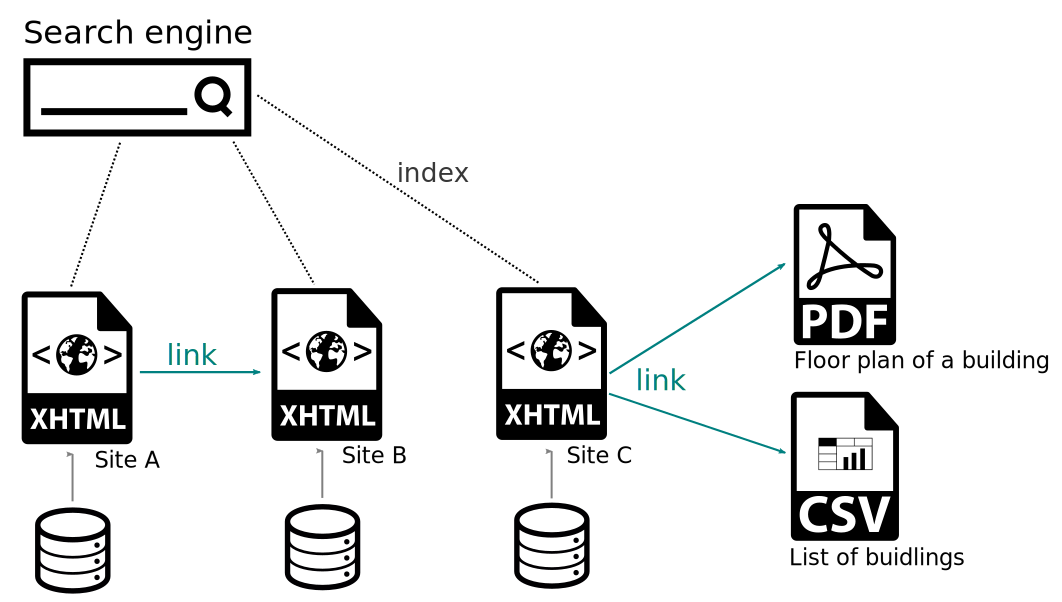
\includegraphics[width=0.75\textwidth]{graphics/webOfDocuments.png}
    \caption{Illustration of the Web of Documents}
    \label{fig:motiviation-web-of-documents}
\end{figure}

The same applies at the moment to the \gls{tuv}. In order to find a special location like a certain lecture hall and how it can be accessed without obstacles like stairways for persons with mobility-impairments, one has to search for information on different web sites, scan floor plans and eventually construct a convenient route to the location based on the gathered knowledge. For humans this procedure does not constitute a problem, but think of machines. The process of information retrieval through data mining or harvesting is quite difficult and/or time consuming. As a consequence application developers that may have innovative ideas, which would be a benefit for the information environment of the university, face a barrier that is hard to overcome. \gls{ld} is one way to transform this information published on multiple web sites into a university-wide data space (see figure \ref{fig:motiviation-web-of-data}).

\begin{figure}[h]
    \centering    
    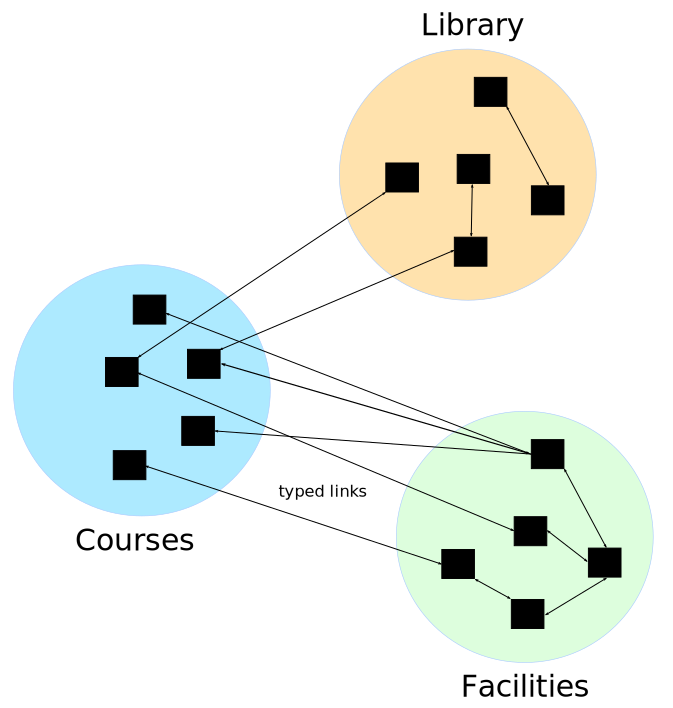
\includegraphics[width=0.5\textwidth]{graphics/webOfData.png}
    \caption{Illustration of the Web of Data}
    \label{fig:motiviation-web-of-data}
\end{figure}

\begin{quote} \gls{ld} describes a method of publishing structured data so that it can be interlinked and become more useful. It builds upon standard Web technologies, but rather than using them to serve web pages for human readers, it extends them to share information in a way that can be read automatically by computers. This enables data from different sources to be connected and queried
\cite{bizer_linked_2009}.\end{quote}

This thesis aims to show the potential that could evolve, if spatial data about \gls{tuv} is transformed into a machine-readable form such as \gls{ld}, by proposing a prototype of a map application based on a subset of spatial data about \gls{tuv}. This subset is intended to comply with the principles of \gls{ld} \cite{berners-lee_linked_2009} and to fulfil the submission criteria to the Linking Open Data cloud\footnote{\url{http://lod-cloud.net/}}, which are as follows \cite{cyganiak_linking_2011}:

\begin{itemize}
	\item There must be resolvable \texttt{http://} (or \texttt{https://}) URIs.
	\item They must resolve, with or without content negotiation, to RDF data in one of the popular RDF formats (RDFa, RDF/XML, Turtle, N-Triples).
	\item The dataset must contain at least 1000 triples.
	\item The dataset must be connected via RDF links to a dataset that is already in the diagram. This means, either your dataset must use URIs from the other dataset, or vice versam. We arbitrarily require at least 50 links.
	\item Access of the entire dataset must be possible via RDF crawling, via an RDF dump, or via a SPARQL endpoint.
\end{itemize}


\section{Problem description}
\label{intro-problem-description}

As already mentioned does the \gls{tuv} distribute spatial information over different sources. Few of this spatial data is actually in a machine-readable format, so that it can be transformed into \gls{ld} automatically. The \textbf{\textit{1st problem}} to solve is therefore the transformation process of the unstructured part of the data into a machine-readable format. Section \ref{solution-data-acquisition} is suggesting a solution for this problem.

The \textbf{\textit{2nd problem}} is how the structured spatial data shall be described so that it can be easily used by application developers as well as integrated into the Web of Data. The developed ontology shall be compliant to the best practises for publishing ontologies \cite{berrueta_best_2008}. Section \ref{solution-ontology-prototype} is suggesting a prototype of an ontology by taking already existing approaches (see section \ref{related-work-geospatial-ontologies} and \ref{related-work-indoor-modelling}) into consideration.

After the spatial data was transformed into \gls{ld}, a system must be designed to expose this data on the Web in order to qualify as \gls{lod}, representing the \textbf{\textit{3rd problem}} to solve. The solution shall take best practises for publishing \gls{ld}\cite{hyland_best_2014} and best practises for spatial data on the Web\cite{tandy_spatial_2016} into consideration. Section \ref{solution-architectural-prototype} is proposing an architectural prototype of such a system.

The \textbf{\textit{4th problem}} is the development of a map application that is based on the resulting \gls{lod}. The application shall answer the following question: \textit{"Give me all learning rooms that are nearby that are free in a given time range and are accessible without obstacles for person with mobility-impairments"} to show the potential of the data. Section \ref{solution-map-application} presents a solution to this problem.

\section{Structure of the thesis}
This chapter outlined the motivation for writing this thesis and gave a description of the problems for which a solution will be suggested. The rest of this thesis is structured as follows: Chapter \ref{background-chapter} discusses the basic concepts, principles and technologies that build the foundation of \gls{ld} and the Semantic Web. It is intended to be a brief introduction for readers that are not familiar with this topic. Chapter \ref{related-work-chapter} provides a summary of past efforts in research and works related to the focus of this thesis. In the subsequent chapter \ref{solution-chapter} a solution for the given problems will be suggested and discussed. This includes the prototype of an ontology that models the problem domain as well as an architectural prototype of a system that manages a subset of spatial data about the \gls{tuv} in form of \gls{ld} and provides a human- and machine-friendly interface to it. Finally, the implemented solution is evaluated and conclusions are drawn in the last chapter \ref{discussion-chapter}. It provides furthermore an outlook to future work and potential improvements. 

\chapter{Background}
\label{background-chapter}

\section{Web of Data}
\todo{Enter your text here.}

\section{RDF}
\gls{rdf}
\todo{Enter your text here.}

\section{Ontology}
\todo{Enter your text here.}

\subsection{RDFS}
\todo{Enter your text here.}

\subsection{OWL}
\todo{Enter your text here.}

\section{SPARQL}
\gls{sparql}
\todo{Enter your text here.}

\chapter{Related Work}
\label{related-work-chapter}

In this chapter important efforts and research related to this thesis are outlined. Section \ref{related-work-geospatial-ontologies} describes and evaluates geospatial ontologies that were suggested by \cite{tandy_spatial_2016} or discovered in the dataset of \gls{lov} through a systematic search. Section \ref{related-work-map-app} lists already existing map applications that are based on \gls{lod} and describes their capabilities. The final section \ref{related-work-indoor-modelling} describes done research and designed ontologies for modelling indoor environments.

\section{Geospatial ontologies}
\label{related-work-geospatial-ontologies}
This section is going to outline common ontologies for describing geospatial data and to evaluate them from the perspective of the given problem description (see \ref{intro-problem-description}).The ontologies were either be suggested by \cite{tandy_spatial_2016} or discovered in the dataset of \gls{lov} by common spatial search terms like \textit{'feature'}, \textit{'geometry'} or \textit{'location'}. \textit{Feature} and \textit{Geometry} are widely used terms in these ontologies and describe two different concepts of geospatial science. A \textit{feature}  is simply a spatial entity that can be everything from a building with fixed position to a movable food truck as long as it has a spatial extent. \textit{Geometry} as the name suggests is a certain geometric shape from points, lines to polygons. Geometric shapes can be used to describe  the spatial extent of \textit{features}.

The ontologies are visualized using the VOWL2 notation\cite{lohmann_vowl_2014}. Classes are modelled as circles, properties in form of rectangles; data type properties have a green colour and object properties a blue one. Literals are presented in a yellow rectangle.

\subsection{Basic Geo Vocabulary (WGS84)}
\label{related-work-geospatial-ontologies-wgs84}

\gls{geo}\cite{brickley_basic_2003} is a lightweight ontology published by W3C to describe the position of a spatial \textit{feature} using the WGS84 geodetic reference datum\footnote{\url{http://en.wikipedia.org/wiki/World_Geodetic_System}} with the properties \texttt{longitude}, \texttt{latitude} and \texttt{attitude}. The general class \texttt{SpatialThing} is the domain of all these properties. Figure \ref{fig:related-work-geospatial-ontologies:wgs84} shows a visualization of this ontology.

\begin{figure}[H]
    \centering    
    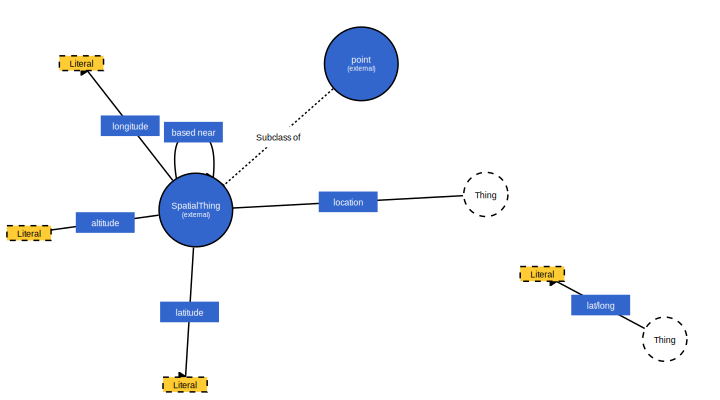
\includegraphics[width=\columnwidth]{graphics/vocabularies/wgs84.png}
    \caption{Visualization of \gls{geo}}
    \label{fig:related-work-geospatial-ontologies:wgs84}
\end{figure}

Advantages are it`s simplicity and popularity as an analysis of the \textit{Comprehensive Knowledge Archive} (CKAN, "The Data Hub"\footnote{\url{http://thedatahub.org}}) indicates. This analysis shows that \gls{geo} is used in \textbf{538} different datasets in the archive and is thereby the 4th most used ontology regarding usage in different datasets \cite{research_group:_akws_lodstats_????}. It is used by big players like DBpedia\footnote{\url{http://dbpedia.org}}, LinkedGeoData\footnote{\url{http://linkedgeodata.org/About}} and GeoNames\footnote{\url{http://linkedgeodata.org/About}}. 
Listing \ref{lst:related-work-geospatial-ontologies:wgs84-dbpedia} shows a data snippet of DBpedia describing the town square 'Karlsplatz' in Vienna with \gls{geo}.

\begin{lstlisting}[frame=single, caption=Snippet of DBpedia, label={lst:related-work-geospatial-ontologies:wgs84-dbpedia}]
@prefix dbr:  <http://dbpedia.org/resource/> .
@prefix geo:  <http://www.w3.org/2003/01/geo/wgs84_pos#> .

dbr:Karlsplatz  rdf:type  geo:SpatialThing ;
  rdfs:label  "Karlsplatz"@en , "Karlsplatz (Wien)"@de ;
  geo:lat     "48.19916534423828125"^^xsd:float ;
  geo:long    "16.370000839233398438"^^xsd:float .
\end{lstlisting}

\gls{geo} evolved into a standard for presenting the location of points of interest and as described by \cite{hyland_best_2014} in an article about best practises, standardized ontologies shall be used wherever possible to facilitate
inclusion into the Web of Data.

However, this ontology is not sufficient for describing spatial data more complex than a single point in a coordinate reference system.

\subsection{NeoGeo Geometry/Spatial Ontology}
\gls{ngeo}\footnote{\url{http://geovocab.org/geometry}} is an ontology that aims to provide a comprehensive descriptive power for modelling geographic regions, whereas \gls{spatial}\footnote{\url{http://geovocab.org/spatial}} aims to describe topological relationships between \textit{features}. Both ontologies were designed to have a strict distinction between \textit{features} and \textit{geometries} \cite{norton_neogeo_2012}.

\subsubsection{\gls{ngeo}} 
\gls{ngeo} follows the principle of modelling geometries in pure \gls{rdf}, which leads to a number of classes and properties for covering all shapes suggested by Simple Features Profile\footnote{\url{http://www.ogcnetwork.net/gml-sf}}. This includes points, lines and polygons. Shapes that go beyond a simple point are represented by a \gls{rdf} collection of \texttt{point} instances, whereby \texttt{point} is a external class of \gls{geo}. Figure \ref{fig:related-work-geospatial-ontologies:ngeo} shows a visualization of this ontology.

\begin{figure}[h]
    \centering
    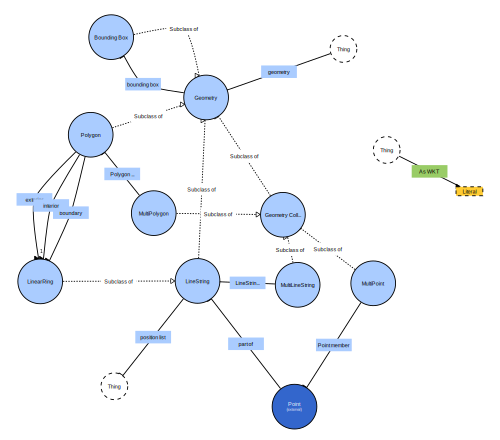
\includegraphics[width=1.0\textwidth]{graphics/vocabularies/geom.png}
    \caption{Visualization of \gls{ngeo}}
    \label{fig:related-work-geospatial-ontologies:ngeo}
\end{figure}

One advantage of this approach is that triple stores do not have to meet special requirements in order to enable the querying over geometric data like it is the case for GeoSPARQL. However, this shifts the burden of writing geometric queries to developers. A further problem is the high demand for resource identifiers or blank nodes (at least for each point of a shape), as the example of describing the geometry of Iceland shows\footnote{\url{http://nuts.geovocab.org/id/IS_geometry.ttl}}; this significantly increases the verbosity of the data without adding particular gains of expressitivity to the data\cite{battle_geosparql:_2011}. \gls{ngeo} has also a generic property \texttt{asWKT} for pointing to the \gls{wkt} serialization of a geometry, which has at the moment of writing the status 'deprecated'.

LinkedGeoData and GeoNames use both the \texttt{geometry} property of this ontology to point to the \textit{geometry} of a \textit{feature}, but use other approaches to represent it.

\subsubsection{\gls{spatial}}
\gls{spatial} is an ontology that aims to provide properties to make topological relationships of \texttt{features} explicit, which else would only exist implicit in the geometric data. Included properties cover all topological relationships described by RCC-8 like does a \textit{feature} overlap with another \textit{feature}. One problem of making the relationships explicit is that these relationships have to be adopted if the \textit{geometry} of \textit{features} changes.

\subsection{GeoSPARQL}
GeoSPARQL defines a set of SPARQL extension functions, a set of \gls{rif} rules, and a core ontology for geographic information\cite{perry_ogc_2012}.

\begin{figure}[h]
    \centering
    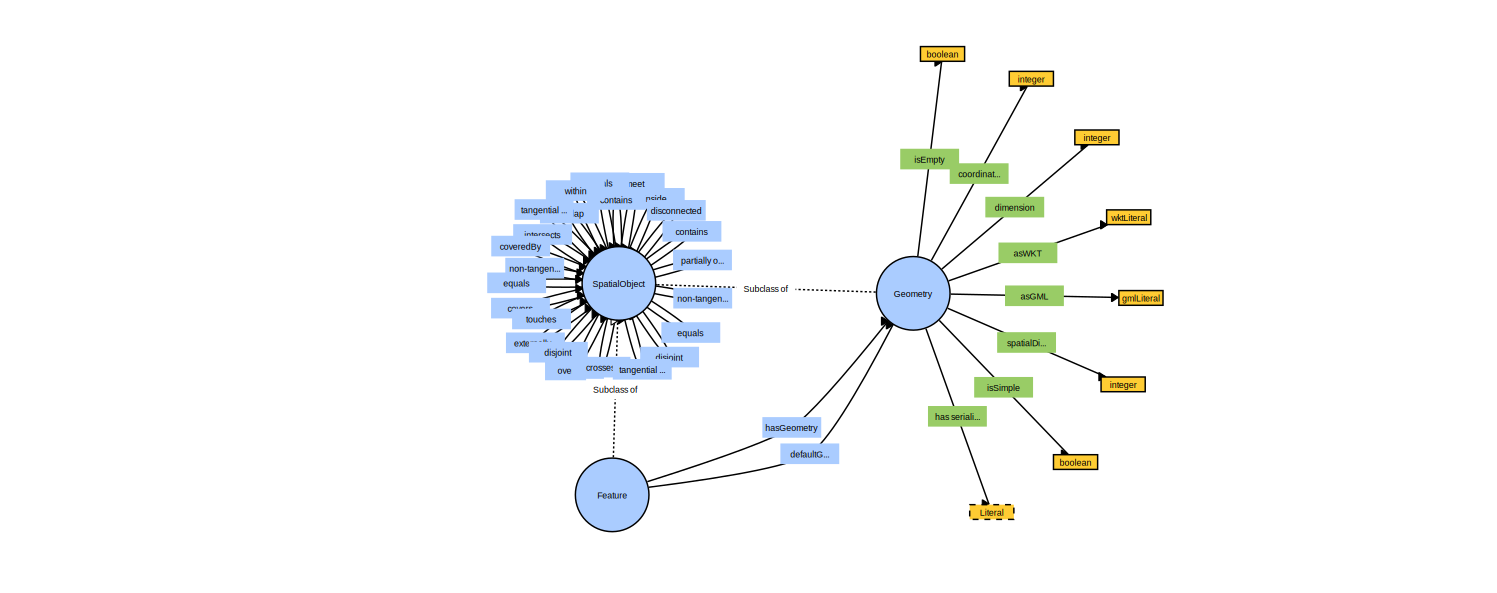
\includegraphics[width=1.0\textwidth]{graphics/vocabularies/geosparql.png}
    \caption{Visualization of GeoSPARQL}
    \label{fig:related-work-geospatial-ontologies:geosparql}
\end{figure}

\subsection{schema.org}
schema.org\footnote{\url{http://schema.org/}} is an initiative that was started by Google, Bing and Yahoo! (subsequently joined by Yandex) to promote a common ontology for publishing structured data mark-up on web pages \cite{guha_introducing_2011}. This machine-readable information can then be extracted from web pages by search engines to improve search results.

schema.org is a quite broad ontology covering a set of different domains from events, organizations to places. For this thesis especially the class \texttt{Place} is of interest describing entities with a fixed, physical extent; it has a set of more specific subclasses. This class has properties to assign an address to it`s instances  (\texttt{address}) as well as to provide geo-information (\texttt{geo}). The value of the property \texttt{geo} can either be instances of the class \texttt{GeoCoordinates} or \texttt{GeoShapes}. \texttt{GeoCoordinates} represents a point in a georeference system similar to \gls{geo}. \texttt{GeoShapes} on the other hand provide the ability to describe more complex geometric shapes including cirlces, boxes, polygons and simple lines. All those shapes are expressed in textual form following an own specific pattern, in contrast to GeoSparql, which declares the use of \gls{gml} or \gls{wkt}. However, such literals could be transformed into \gls{wkt} by string operations (supported in \gls{sparql}) except for the circle, which has no direct representation in \gls{wkt}.

One advantage of this ontology is the visibility to search engines when exposed on web pages in one of the supported formats (Microdata\footnote{\url{https://www.w3.org/TR/microdata/}}, \gls{rdfa}\footnote{\url{https://www.w3.org/TR/rdfa-syntax/}} and JSON-LD\footnote{\url{http://json-ld.org/}}). As mentioned earlier, the embedded data can then be extracted and in fact major search engines crawl for it to enhance search results\cite{haas_enhanced_2011}. \todo{mention function}. There are furthermore odd ascriptions of properties  like that instances of the class \texttt{Beach} (subclass of \texttt{Place}) can have the property \texttt{faxNumber}; it must be considered that schema.org is meant for web masters to add structured metadata to their web sites \cite{veres_schema.org_2013} and not to describe a specific domain precisely.

\subsection{ISA Programme Location Core Vocabulary}
\gls{locn} is an ontology that provides a set of properties and classes to describe the geometry, address and location of a \textit{feature}. Figure \ref{fig:related-work-geospatial-ontologies:locn} shows a visualization of this ontology. It provides a comprehensive set of properties to describe the address of a \textit{feature}, but a mininal set for geometries and locations. For geometries this ontology suggests the use of external classes or a simple literal representing the serialization of the geometry in formats such as \gls{wkt} and \gls{gml}. Those suggested classes are \textit{Geometry} of GeoSPARQL with it`s more specific subclasses and \texttt{GeoCoordinates} as well as \texttt{GeoShapes} from schema.org. In case of representing simple points also \texttt{point} of \gls{geo} is mentioned. \cite{perego_isa_2015} Howerver, this quite broad range of possibilities does not make it easy for the consumer of such \gls{ld}.

\begin{figure}[h]
    \centering
    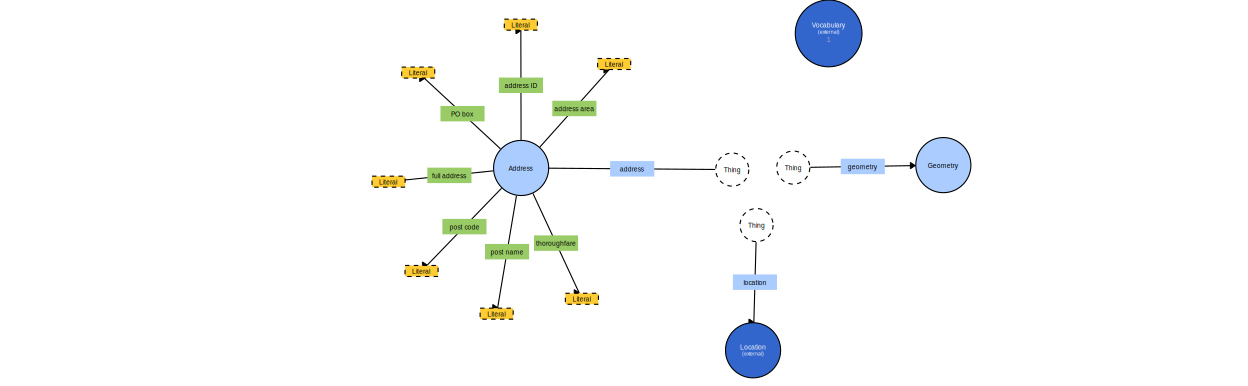
\includegraphics[width=1.0\textwidth]{graphics/vocabularies/locn.png}
    \caption{Visualization of \gls{locn}}
    \label{fig:related-work-geospatial-ontologies:locn}
\end{figure}

\subsection{Other ontologies}
\label{related-work-other-ontologies}


\section{Linked Open Data based map applications}
\label{related-work-map-app}

Multiple universities (e.g. Linked Universities\footnote{\url{http://linkeduniversities.org}}) exposed their public university data and map applications played out to be a common use case for this data.

University of Münster started an Open Data initiative named LODUM\cite{kesler_linked_2012} from which a map application\footnote{\url{http://app.uni-muenster.de/Karte/}} evolved that shows the location of buildings and which departments are located in the selected building, but there is no deeper insight into the buildings. However, there is a publication of the initiative that deals with the issue of indoor navigation \cite{kostic_automated_2015-1}. Furthermore an indoor map ontology was designed (see section \ref{related-work-indoor-modelling-limap}).

University of Southampton is a further university that exposed spatial information about their campus as \gls{lod}. In contrast to the map of the LODUM initiative Southampton`s map application\footnote{\url{http://maps.southampton.ac.uk/}} (see figure \ref{fig:related-work-map-app:southampton}) gives insight into buildings and shows the location of certain rooms with the ability to switch the floor. It shows also computer rooms with their current estimated capacity and opening hours.  

\begin{figure}[h]
    \centering
    \includegraphics[width=0.75\textwidth]{graphics/maps/southampton-map-app.png}
    \caption{Map application of University of Southampton}
    \label{fig:related-work-map-app:southampton}
\end{figure}

University of Oxford has also exposed spatial information in form of \gls{lod} on their Open Data portal and developed an application named \textit{University Science Area Map} \footnote{\url{https://data.ox.ac.uk/explore/science-area/}}. It highlights buildings, where departments of a certain field are located, on a map, but it gives no insight into the buildings.

\section{Indoor modelling}
\label{related-work-indoor-modelling}
Section \ref{related-work-geospatial-ontologies} outlined ontologies to describe the spatial extent of \textit{features} and topological relationships between them, but those ontologies are not intended for expressing the characteristics of \textit{features} in an indoor environment; like for example that a \textit{feature} is a learning room with certain opening hours or an elevator to get from one floor to another. This section discusses ontologies to model indoor environments that have been discovered in the repository of \gls{lov} by searching for terms such as \textit{'room'}, \textit{'building'} and \textit{'toilette'} or explored in datasets of map applications based on \gls{lod} (see section \ref{related-work-map-app}).

\subsection{LIMAP}
\label{related-work-indoor-modelling-limap}

\begin{figure}[h]
    \centering
    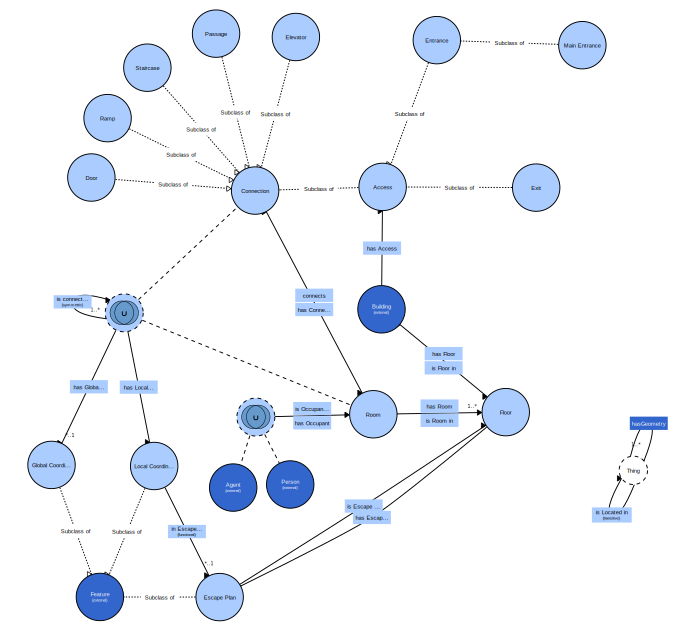
\includegraphics[width=1.0\textwidth]{graphics/vocabularies/limap.png}
    \caption{Visualization of \gls{limap}}
    \label{fig:related-work-geospatial-ontologies:locn}
\end{figure}

\subsection{Other ontologies}
\label{related-work-indoor-modelling-other-ontologies}
\gls{rooms} provides a minimal set of classes and properties to describe the basic structure of a building. It has 6 classes \texttt{Building}, \texttt{Floor}, \texttt{FloorSection}, which is a named (identifiable) section of a floor,\texttt{Room} and \texttt{Desk} as well as \texttt{Site}, which describes an area of land like a campus.


\chapter{Solution}
\label{solution-chapter}

This chapter suggests solutions for the given problem description (see \ref{intro-problem-description}). Section \ref{solution-data-acquisition} is dealing with the problem of transforming unstructured spatial data about the \gls{tuv} into a machine-readable format. The question of how this structured data shall be described is answered in section \ref{solution-ontology-prototype}, where a prototype of an ontology is discussed. The subsequent section \ref{solution-architectural-prototype} is proposing an architectural prototype of a system for integrating and publishing \gls{ld} consistent with the \gls{ld} principles \cite{berners-lee_linked_2009}. The final section \ref{solution-map-application} is presenting a map application to show the potential of the generated spatial \gls{lod}.

\section{Data acquisition}
\label{solution-data-acquisition}
Spatial data about the \gls{tuv} is distributed over multiple sources with different formats and data owners. In order to be eventually transformed into \gls{ld}, this data must be extracted and prepared for the integration. Figure \ref{fig:solution-data-acquisition:sources} visualizes the different data sources.

The major source for building information is the web site of the facility management unit of the \gls{tuv} (GUT\footnote{\url{http://www.gut.tuwien.ac.at/}}). This site lists all buildings and an enumeration of their floors in form of a (X)HTML table. It also contains links to the floor plans that are provided as \gls{pdf} files as well as to a \gls{pdf} file for each building consisting of a table of all contained rooms with their intended function (e.g. office room, sanitary room). Section \ref{solution-data-acquisition-tables} deals with the problem of extracting and transforming tables from \gls{pdf}s and web pages. The approach for processing floor plans is discussed in section \ref{solution-data-acquisition-floor-plans}.


The central information system TISS\footnote{\url{https://tiss.tuwien.ac.at/}} provides a RESTful API that gives access to organizational information and the public address book. For this thesis, this API is useful for linking persons and organizations to their offices. TISS has also a web page dedicated to presenting the event schedule of certain rooms like lecture halls, but this data is not available over the mentioned RESTful API; only in a human-readable form. 


\begin{figure}[h]
    \centering
    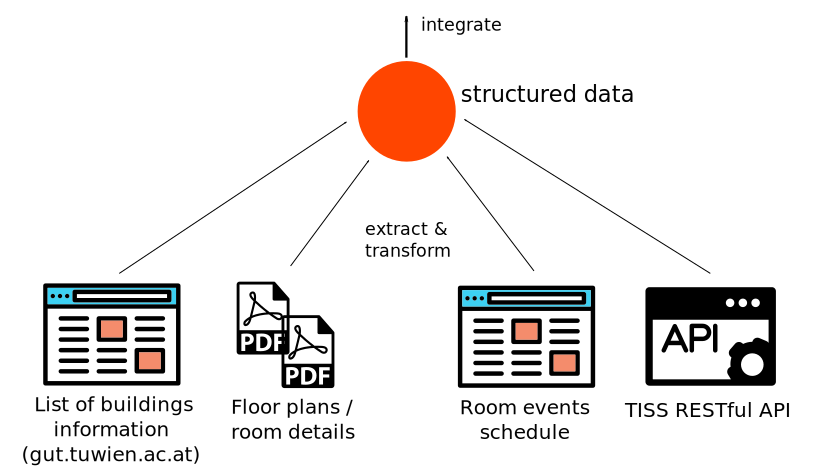
\includegraphics[width=0.75\textwidth]{graphics/dataAcquisitionSources.png}
    \caption{Visualization of the data sources}
    \label{fig:solution-data-acquisition:sources}
\end{figure}


\subsection{(X)HTML and \gls{pdf} tables}
\label{solution-data-acquisition-tables}
As mentioned earlier, some of the data is presented to users only in form of (X)HTML tables and must therefore be extracted in order to be transformed into \gls{ld}. Web scrapers/Web harvester are an useful tool to extract such tables from web pages manually or by using XPATH expressions and to store them in an intermediate representation. For this thesis a chrome extension named 'Web Scraper' \footnote{\url{http://webscraper.io/}} was used. This intermediate representation was then exported into a \gls{csv} file.

For tables in \gls{pdf} files a different approach is required and the tool named 'Tabula'\footnote{\url{http://tabula.technology/}} is qualified for this kind of problem. It can detect tables automatically and transforms them into an intermediate representation, but this does not always work appropriately. In this case, the user can support the program by selecting the relevant parts manually. This intermediate representation was then also exported into a \gls{csv} file.

After the information was extracted from web pages and \gls{pdf} files and transformed into a structured format, it still was messy data that is not convenient for a further transformation into \gls{ld}. In this case the tool OpenRefine\footnote{\url{http://openrefine.org/}} is quite useful. It provides a set of abilities to manipulate messy, tabular data including an own expression language named GREL. LODRefine and RDF extension are extensions for OpenRefine, which enable the transformation of tabular data into \gls{rdf} by mapping columns to classes and relationships between columns to properties. This mapping is then computed for each row. 

\subsection{Floor plans}
\label{solution-data-acquisition-floor-plans}
Floor plans are ideal for describing the internal structure of a building, but they are mostly available in form of images and vector graphics. This representation is fine for humans, but not for machines; because the floor plan should not only be available as single image, but rather be the knowledge base for applications to find paths and locate rooms in the corresponding building.

Google Maps is a map application that also gives insight into certain buildings. It provides a tool \footnote{\url{https://maps.google.com/floorplans/find}}, where any user can submit floor plans and this floor plan then will be automatically transformed into an internal representation that can thenceforward be looked at in the application (if accepted). The problem is that the user cannot demand access to this internal representation of the plan, although the user may be the owner. Figure \ref{fig:solution-data-acquisition:tuvienna-lib-gm-indoor} shows the indoor plan of \gls{tuv}`s main library in Google Maps.

\begin{figure}[h]
    \centering
    \includegraphics[width=0.75\textwidth]{graphics/google-maps-tu-vienna-library-indoor-plan.png}
    \caption{Google Maps: Indoor plan of \gls{tuv}`s main library}
    \label{fig:solution-data-acquisition:tuvienna-lib-gm-indoor}
\end{figure}

Due to the lack of alternatives, the approach used for this thesis was to manually transform two floor plans of one building into shape files. The tool used for this approach was the Open Source software QGIS\footnote{\url{http://www.qgis.org/}}. It has two plugins that are useful for the transformation, the 'Open Layers' plug-in to enable the use of OpenStreetMaps among others and the GDAL georeferencing plug-in to position a raster image on a map. Especially the last plug-in is important for positioning the floor plan to the correct position on the map, whereby the map should already contain the boundary of the building. After georeferencing the floor plan, a shape file of the rooms and other \textit{features} of interest can be created. Each of the created shapes has a table of attributes with an unique ID that can be set by the user. The unique ID of each shape is an \gls{iri}, so that the shape is ready to be transformed into \gls{ld}. The resulting shape file can then be exported in multiple formats including GeoJSON\footnote{\url{http://geojson.org/}}. For this thesis, a \gls{csv} file with the \gls{wkt} serialization of each shape of the file and the corresponding ID per row showed to be the easiest way to integrate this data. Figure \ref{fig:solution-data-acquisition:tuvienna-lib-gm-indoor} shows a shape file of rooms on the basement floor of the informatics institute`s building at the \gls{tuv}.

\begin{figure}[h]
    \centering
    \includegraphics[width=0.75\textwidth]{graphics/qgis-floor-plan-building-h-eg.png}
    \caption{Room shapes file of the basement floor of the informatics institute`s building}
    \label{fig:solution-data-acquisition:tuvienna-lib-gm-indoor}
\end{figure}

\subsection{XML}
\label{solution-data-acquisition-tables}

\todo{Describe ... }

\section{Prototype of ontology}
\label{solution-ontology-prototype}
\todo{Description of the developed ontology with newly created terms and reused ones, and why using GeoSPARQL and what are the disadvantages}

\section{Architectural prototype}
\label{solution-architectural-prototype}
\todo{A description of the system, the different layers, integration, linking and web framework, REST API, used technologies}

\subsection{System architecture}
\todo{Description of the system architecture}

\subsection{RDF Framework}
\todo{Reasoning why using Sesame, not Apache Jena}

\subsection{Linked Data management}
\todo{Description of the data management and compliance to best practise}

\subsection{Linking}
\todo{Description of strategies for linking with external sources and to enrich the data}

\subsection{Linked Data publishing}
\todo{Description of the data publishing and compliance to best practise}

\section{Map application}
\label{solution-map-application}
\todo{A more comprehensive presentation of the user interface for humans to show the targeted use case.}

\chapter{Discussion}
\label{discussion-chapter}

\section{Evaluation}
\todo{Enter your text here.}

\section{Further work}
\todo{Enter your text here.}

\section{Conclusion}

\todo{Enter your text here.}

\backmatter

% Use an optional list of figures.
\listoffigures % Starred version, i.e., \listoffigures*, removes the toc entry.

% Use an optional list of tables.
\listoftables % Starred version, i.e., \listoftables*, removes the toc entry.

% Use an optional list of alogrithms.
\listofalgorithms
\addcontentsline{toc}{chapter}{List of Algorithms}

% Add an index.
\printindex

% Add a glossary.
\printglossaries

% Add a bibliography.
\bibliographystyle{plain}
\bibliography{thesis}

\end{document}